\documentclass[12pt]{article}
% Based on the supplied latex_template.tex: 12pt article, A4, one-inch margins.
\usepackage{graphicx}
\usepackage{amsmath}
\usepackage{amsthm}
\usepackage{amssymb}
\usepackage{amsfonts}
\usepackage{enumerate}
\usepackage{array}
\usepackage[hidelinks]{hyperref}
\usepackage[a4paper,margin=1in]{geometry}
\IfFileExists{setspace.sty}{\usepackage{setspace}}{}
\newcommand{\R}{\mathbb{R}}
\newcommand{\N}{\mathbb{N}}
\newcommand{\Q}{\mathbb{Q}}
\newcommand{\Z}{\mathbb{Z}}
\theoremstyle{definition}
\newtheorem{theorem}{Theorem}
\newtheorem{corollary}{Corollary}
\newtheorem{definition}{Definition}
\newtheorem{example}{Example}
\newtheorem{exercise}{Exercise}
\newcommand{\E}{\mathbb{E}}
\newcommand{\Var}{\operatorname{Var}}
\newcommand{\ind}{\mathbf{1}}
\setlength{\parindent}{0pt}
\setlength{\parskip}{5pt}
\setlength{\textfloatsep}{10pt}
\setlength{\intextsep}{8pt}
\setlength{\abovedisplayskip}{7pt}
\setlength{\belowdisplayskip}{7pt}
\renewcommand{\arraystretch}{1.13}
\title{Monte Carlo and Finite Difference Methods\\for Option Pricing}

\date{}
\begin{document}
% Public portfolio report title.
\begin{center}
{\Large\bfseries Monte Carlo and Finite Difference Methods\\[3pt]
for Option Pricing: A Numerical Investigation}
\end{center}


\section{Questions and experimental design}
The two contracts create different numerical difficulties. The digital payoff jumps at
the strike, whereas the barrier call can be knocked out between simulated dates.
I compare Monte Carlo (MC) and finite differences by separating sampling error
from discretisation effects.
The risk-neutral model and parameters are
\[
dS_t=rS_t\,dt+\sigma S_t\,dW_t,\qquad
(S_0,r,\sigma,T)=(100,0.05,0.25,1).
\]
For Extension B, I test whether a geometric control variate makes arithmetic Asian
pricing more efficient once its extra simulation cost is included.

\begin{center}
\setlength{\tabcolsep}{4pt}
\begin{tabular}{|>{\raggedright\arraybackslash}p{1.9cm}|>{\raggedright\arraybackslash}p{3.5cm}|>{\raggedright\arraybackslash}p{3.7cm}|>{\raggedright\arraybackslash}p{5.3cm}|}
\hline
\textbf{Problem}&\textbf{Methods used}&\textbf{Investigation}&\textbf{Main conclusion}\\\hline
Digital&Standard, antithetic and importance-sampled MC; explicit, implicit and CN finite differences (FD)&Equal simulation budgets; payoff averaging; grid convergence and stability&Importance sampling improves MC at $K=140$. Averaged CN with implicit startup gives much smaller errors at comparable cost.\\\hline
Barrier&Discrete and bridge MC; explicit, implicit and CN FD&Missed crossings; a boundary at the barrier; accuracy versus runtime&Discrete monitoring overprices. Use bridge conditioning for simulation and damped CN for high precision.\\\hline
Asian (B)&Standard MC and a geometric control variate&Variance reduction, independent validation and cost&At one million paths, the control reduces variance about 835-fold. The gain remains substantial after allowing for pilot cost.\\\hline
\end{tabular}
\end{center}

\textbf{Design and reproducibility.}
MC samples are generated from the model, and FD prices are computed on a grid.
The accompanying Python program saves the results, seeds and figures. It uses Python 3.13.7, NumPy 2.3.3
and SciPy 1.16.2 on Windows, with base seed 20260914 and separate experiment offsets.
Reported runtimes are medians of three complete calls, excluding plotting and file
output; Asian control timings include the independent pilot. They measure this
implementation on this machine.

For independent discounted observations $Y_i$, I report their mean, standard error
$\mathrm{SE}=s_Y/\sqrt n$ and approximate 95\% interval
$\overline Y\pm1.96\mathrm{SE}$. An antithetic pair is one observation. FD error is
measured against a known or independently evaluated benchmark. Replicated MC runs
avoid judging accuracy from one fortunate estimate; successive grid refinements
check whether FD results have settled.

\newpage
\section{Digital call: simulation and variance reduction}
The digital pays $\ind_{\{S_T>140\}}$. Write $\mu=r-\sigma^2/2$ and
$a=[\log(K/S_0)-\mu T]/(\sigma\sqrt T)$. Exact terminal simulation uses
\[
S_T=S_0\exp(\mu T+\sigma\sqrt T Z),\quad Z\sim N(0,1),\qquad
V_D=e^{-rT}\Phi(-a)=0.0969151345.
\]
Here $\Phi$ is the standard normal distribution function. The exercise probability is
only $p=\Phi(-a)\simeq0.1019$, so most standard samples contribute zero. There is no
time discretisation error because only the terminal stock price is needed.

I compare the sampling methods at a fixed payoff budget.
Antithetic MC averages the payoffs obtained from $Z$ and $-Z$. For importance sampling
(IS), draw $Z\sim N(0,1)$ and shift to $X=Z+a$. The observation is
\[
Y_{\rm IS}=e^{-rT}\ind_{\{X>a\}}\exp(-aZ-a^2/2).
\]
The exponential is the original normal density divided by the shifted density, so the
expectation is unchanged. The threshold lies at the new mean and half the samples
exercise. This simple shift is held fixed as a rule; it is not claimed to be optimal.

\begin{center}
\begin{tabular}{lrrrr}
\hline
Method&Price&SE&95\% half-width&Time (s)\\\hline
% BEGIN GENERATED digital_mc
Standard & 0.096970 & 0.000288 & 0.000564 & 0.0252 \\
Antithetic & 0.097482 & 0.000272 & 0.000532 & 0.0222 \\
IS & 0.096795 & 0.000125 & 0.000245 & 0.0516 \\
% END GENERATED digital_mc
\hline
\end{tabular}

Table 1: $10^6$ payoff evaluations; antithetic uses $5\times10^5$ pairs.
\end{center}

The estimated equal-budget variance reductions are 1.12 for antithetic and 5.28 for IS.
Counting pairs correctly matters: comparing the observation variances alone would
overstate the antithetic gain by a factor of two. IS costs more per sample but reduces
$\mathrm{SE}^2\times\text{runtime}$ by 2.57 relative to standard MC.

\begin{center}
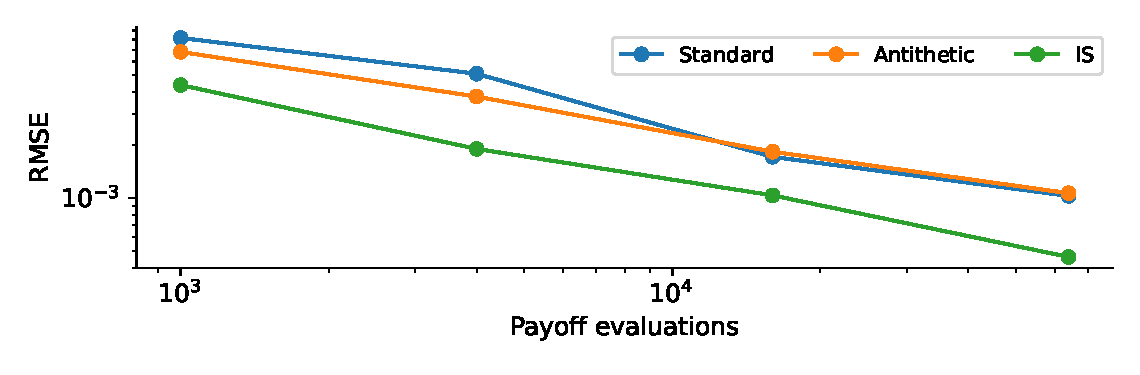
\includegraphics[width=0.88\linewidth]{figures/digital_mc.pdf}

Figure 1: RMSE from 40 independent runs at each simulation budget.
\end{center}

Budgets $10^3,4\times10^3,1.6\times10^4,6.4\times10^4$ give log--log slopes
$-0.53,-0.45,-0.53$ for standard, antithetic and IS respectively. The results are
consistent with $n^{-1/2}$ convergence: IS improves the constant, not the rate.
The standard estimate in Table 1 happens to be closer to the exact price than IS;
the SEs and repeated runs show why this is not evidence that standard MC is better.
The antithetic interval misses the benchmark in this run, which can occur with a
nominal 95\% interval.

\newpage
\section{Finite differences: the digital discontinuity}
With $u(\tau,S)=V(T-\tau,S)$, the pricing equation is
$u_\tau=\frac12\sigma^2S^2u_{SS}+rSu_S-ru$.
On $S_j=j\Delta S$, central differences give
\[
(L_hu)_j=a_ju_{j-1}+b_ju_j+c_ju_{j+1},\qquad
\begin{cases}
a_j=(\sigma^2j^2-rj)/2,\\
b_j=-\sigma^2j^2-r,\\
c_j=(\sigma^2j^2+rj)/2.
\end{cases}
\]
The time update, with boundary contributions at the appropriate time levels, is
\[
(I-\theta\Delta\tau L_h)u^{n+1}=(I+(1-\theta)\Delta\tau L_h)u^n.
\]
Explicit Euler, implicit Euler and Crank--Nicolson (CN) use $\theta=0,1,1/2$.
I also test Rannacher-started CN (R-CN): replace the first full step by two implicit
half-steps, then use CN \cite{giles}. Each implicit update is a tridiagonal solve.

To test how the discontinuity affects grid convergence, I use $S\in[0,400]$, with $u(\tau,0)=0$ and
$u(\tau,400)=e^{-r\tau}$. The tested grids include both $S_0$ and $K$.
Pointwise terminal data assign zero at $K$; cell averaging assigns $1/2$ there.
Although changing one point does not affect the continuous expectation, a grid node
has a finite numerical weight.

\begin{center}
\setlength{\tabcolsep}{4pt}
\begin{tabular}{rrrrr}
\hline
$M=N$&Raw R-CN error&Averaged error&Implicit error&R-CN (s)\\\hline
% BEGIN GENERATED digital_fd
100 & $9.60\times10^{-3}$ & $3.80\times10^{-5}$ & $3.37\times10^{-4}$ & 0.008 \\
200 & $4.82\times10^{-3}$ & $9.36\times10^{-6}$ & $1.81\times10^{-4}$ & 0.015 \\
400 & $2.41\times10^{-3}$ & $2.33\times10^{-6}$ & $9.37\times10^{-5}$ & 0.038 \\
800 & $1.21\times10^{-3}$ & $5.82\times10^{-7}$ & $4.76\times10^{-5}$ & 0.076 \\
1600 & $6.04\times10^{-4}$ & $1.46\times10^{-7}$ & $2.40\times10^{-5}$ & 0.222 \\
% END GENERATED digital_fd
\hline
\end{tabular}

Table 2: $M$ spatial intervals and $N$ time steps; implicit data are averaged.
\end{center}

Raw-payoff errors approximately halve, whereas averaged R-CN errors fall by four
per doubling. Implicit Euler is approximately first order along $N=M$ because of its
time error. The finest averaged price is $0.096915280$. Keeping $\Delta S=0.5$ and
$N=800$, increasing the upper boundary to 600 and 800 changes the price by less than
$10^{-12}$. Domain truncation therefore does not explain this refinement pattern.

\textbf{Stability and cost.} Here $a_j,c_j\geq0$, and explicit Euler is monotone if
$\Delta\tau[\sigma^2(M-1)^2+r]\leq1$. At $M=400$, $N=12000$ gives ratio 0.829 and
a bounded solution; $N=9000$ gives 1.106 and values exceeding $10^{100}$.
Using $N=\lceil T[\sigma^2(M-1)^2+r]/0.9\rceil=11056$ leaves a safety margin
and gives error $5.94\times10^{-6}$ in 0.485 s.
R-CN uses only 400 steps, giving $2.33\times10^{-6}$ in 0.038 s.

With $M=400,N=20$, plain CN has two local decreases near the strike after its first
step; R-CN removes both. Stability alone does not prevent oscillations. I recommend
averaged R-CN for numerical precision: at $M=200$ its error is already
$9.36\times10^{-6}$ in 0.015 s, below the million-sample IS standard error.
For this particular contract, the closed-form price remains the simplest choice.

\newpage
\section{Barrier call: missed crossings in Monte Carlo}
The up-and-out call has $K=100$, $H=130$ and discounted payoff
\[e^{-rT}(S_T-K)^+\ind_{\{\max_{0\leq t\leq T}S_t<H\}}.\]
Checking the barrier only at simulated endpoints accepts some paths that crossed
$H$ between dates. With a nonnegative payoff this creates upward bias.

I use exact lognormal increments to isolate missed crossings from Euler or Milstein
path discretisation error. For log endpoints $x_i,x_{i+1}<h=\log H$, the
conditional survival probability is \cite{bridge}
\[
q_i=1-\exp\!\left(-\frac{2(h-x_i)(h-x_{i+1})}{\sigma^2\Delta t}\right),
\qquad Y_B=e^{-rT}(S_T-K)^+\prod_i q_i.
\]
Set $q_i=0$ if either endpoint reaches the barrier. Under the specified constant
coefficients, this Brownian bridge weighting removes monitoring bias exactly.
The payoff otherwise depends only on $S_T$, so one interval across $[0,T]$ suffices.

For an independent benchmark, put $x=\log S_0$, $v=\sigma^2T$, and let $\phi_v$
denote the centred normal density with variance $v$. The reflection principle gives
the density of the log price before hitting $h$:
\[
f_{\rm kill}(y)=\phi_v(y-x-\mu T)
-e^{2\mu(h-x)/\sigma^2}\phi_v(y+x-2h-\mu T).
\]
Then $V_B=e^{-rT}\int_{\log K}^{h}(e^y-K)f_{\rm kill}(y)\,dy
=2.2235389914$. Numerical quadrature with absolute and relative tolerances
$10^{-12}$ agrees with direct integration of the bridge-weighted payoff within
$10^{-11}$. This provides a check separate from the FD solver.

\begin{center}
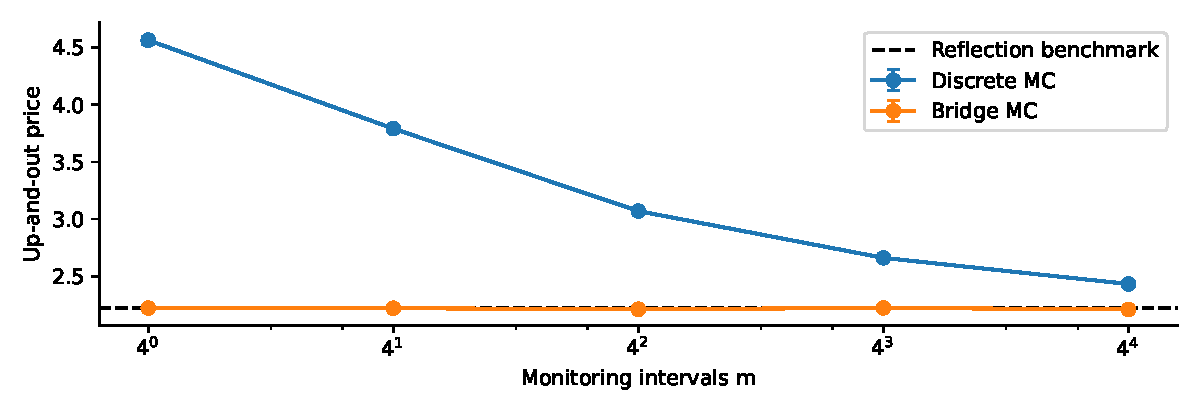
\includegraphics[width=0.96\linewidth]{figures/barrier_monitoring.pdf}

Figure 2: 200,000 paths per resolution; bars show 95\% sampling intervals.
Discrete and bridge estimators use the same increments at each resolution.
\end{center}

At 256 intervals, discrete monitoring gives $2.431888$, an error of $0.208349$,
against SE $0.012288$. The paired discrete-minus-bridge gap is $0.221800$ with
SE $0.004065$, so sampling variation cannot plausibly explain it. The gap falls from
$0.8585$ to $0.4377$ to $0.2218$ at 16, 64 and 256 intervals: approximately halving
when the step size quarters, consistent with a square-root monitoring error.
More paths alone cannot remove this bias.

All five bridge intervals contain the benchmark. Their fluctuations reflect sampling
error, without the systematic downward trend of discrete monitoring. A narrow MC
interval is therefore insufficient evidence of accuracy unless monitoring bias is also
controlled.

\newpage
\section{Barrier efficiency and the Asian extension}
\textbf{Barrier FD.} The grid ends at $H$, with $u(\tau,0)=u(\tau,H)=0$ and
terminal data $(S-K)^+$ for $S<H$. The absorbing boundary kills the option as
soon as the stock reaches $H$. Each grid includes $S_0,K,H$. The terminal payoff
jumps from almost 30 to zero at $H$, which can cause startup oscillations.

\begin{center}
\setlength{\tabcolsep}{5pt}
\begin{tabular}{rrrrr}
\hline
$M=N$&R-CN price&Absolute error&Time (s)&CN minimum\\\hline
% BEGIN GENERATED barrier_fd
130 & 2.2218891 & $1.65\times10^{-3}$ & 0.009 & -1.11 \\
260 & 2.2231267 & $4.12\times10^{-4}$ & 0.022 & -7.21 \\
520 & 2.2234359 & $1.03\times10^{-4}$ & 0.045 & -12.58 \\
1040 & 2.2235132 & $2.58\times10^{-5}$ & 0.096 & -16.98 \\
% END GENERATED barrier_fd
\hline
\end{tabular}

Table 3: CN minimum is taken over every grid node and time level.
\end{center}

R-CN stays nonnegative and its error falls by about four per grid doubling.
Plain CN has similar final accuracy, but the negative intermediate prices in
Table 3 are unrealistic. At $M=520$, explicit Euler takes 0.701 s and 18,706 steps
for error $1.83\times10^{-4}$; R-CN takes 0.045 s and 520 steps for
$1.03\times10^{-4}$. The implicit startup therefore improves the solution at little cost.

One-step bridge MC with $10^6$ paths gives $2.221161$ (SE $0.00342$) in 0.142 s.
R-CN at $M=N=1040$ takes 0.096 s for error $2.58\times10^{-5}$, so I prefer FD
for precision here. For simulation, one bridge interval is enough: at 200,000 paths,
using 256 intervals instead of one raises runtime from 0.025 to 6.179 s and payoff
variance from 11.69 to 25.68. Conditioning only on $S_T$ averages out the extra
randomness in intermediate states, explaining the lower variance.

\textbf{Extension B: a geometric control for the Asian call.}
The contract has $K=100$ and $m=12$ monthly observations. To state the formulas
generally, take $m$ equally spaced dates $t_i=iT/m$, $i=1,\ldots,m$, and define
$A=m^{-1}\sum_i S_{t_i}$ and $G=(\prod_i S_{t_i})^{1/m}$. Neither average includes
$S_0$. The discounted payoffs are $X=e^{-rT}(A-K)^+$ and $C=e^{-rT}(G-K)^+$.
I use $C$ as a control because the two averages respond similarly to a stock path
and $\E[C]$ is known \cite{control}.

$\log G$ averages Gaussian log prices, so it is Gaussian. Using
$\operatorname{Cov}(W_{t_i},W_{t_j})=\min(t_i,t_j)$ gives its mean and variance:
\begin{align*}
m_G&=\log S_0+\mu T\frac{m+1}{2m},\\
v_G&=\frac{\sigma^2}{m^2}\sum_{i=1}^m\sum_{j=1}^m\min(t_i,t_j)
=\sigma^2T\frac{(m+1)(2m+1)}{6m^2}.
\end{align*}
The last equality uses $t_i=iT/m$ and
$\sum_{i,j}\min(i,j)=m(m+1)(2m+1)/6$. Setting $m=12$ gives
$v_G=0.0235098380$; the factors 13 and 25 are simply $m+1$ and $2m+1$.
With $d_2=(m_G-\log K)/\sqrt{v_G}$ and $d_1=d_2+\sqrt{v_G}$,
\[
c_G=\E[C]=e^{-rT}\{e^{m_G+v_G/2}\Phi(d_1)-K\Phi(d_2)\}=6.99073142.
\]
The controlled payoff is $Y=X-\widehat\beta(C-c_G)$. I estimate
$\widehat\beta=\widehat{\operatorname{Cov}}(X,C)/s_C^2=1.039867$ from 20,000
independent pilot paths and keep it fixed for all three production budgets.
Independence gives $\E[Y\mid\widehat\beta]=\E[X]$. Exact simulation at the monthly dates avoids time discretisation bias.

\newpage
\section{Asian results and conclusions}
\begin{center}
\setlength{\tabcolsep}{5pt}
\begin{tabular}{rlrrrr}
\hline
Paths&Method&Price&SE&Time (s)&VR factor\\\hline
% BEGIN GENERATED asian
10,000 & Standard & 7.255985 & 0.106835 & 0.005 & 1.0 \\
10,000 & Geo. CV & 7.308936 & 0.003503 & 0.016 & 929.9 \\
100,000 & Standard & 7.278630 & 0.033557 & 0.048 & 1.0 \\
100,000 & Geo. CV & 7.310995 & 0.001155 & 0.054 & 843.8 \\
1,000,000 & Standard & 7.302458 & 0.010629 & 0.565 & 1.0 \\
1,000,000 & Geo. CV & 7.312727 & 0.000368 & 0.699 & 835.0 \\
% END GENERATED asian
\hline
\end{tabular}

Table 4: $\widehat{\mathrm{VR}}=s_X^2/s_Y^2$ at equal production counts.
CV timings include the 20,000-path pilot; both methods use the same production paths.
\end{center}

The controlled price at $10^6$ paths is $7.312727$, with 95\% interval
$[7.312006,7.313448]$. An independent joint-normal simulation using Cholesky
factorisation gives $7.312286$ (SE $0.000260$) from two million paths. The estimates
differ by less than one combined SE; this is a statistical check, not an exact benchmark.

The decline in the estimated VR factor from 929.9 to 835.0 needs some care.
With the same fixed $\widehat\beta$, both estimators' variances scale as $1/n$, so
their population ratio does not depend on $n$. Table 4 instead uses sample
variances. From $10^4$ to $10^6$ paths, $s_X^2$ changes from 114.136 to 112.984,
while $s_Y^2$ rises from 0.12274 to 0.13531. The smaller run therefore gives a
higher ratio, mainly because it estimates a smaller residual variance. The runs use
different production seeds. These three values do not establish a downward trend
in the method's effectiveness; even at $10^6$ paths, SE is about 29 times smaller.

Including pilot time, the variance--runtime gain is about 278 at $10^4$ paths and
675 at $10^6$: the fixed pilot cost matters less in larger runs. Across 80 further
runs with new pilots, the controlled-price standard deviation is 0.00372, close to
the RMS reported SE of 0.00367.

\textbf{Why FD becomes harder.} The Asian value depends on $S$ and the accumulated
sum $B$. Between observation dates, it satisfies the Black--Scholes PDE in $S$
with $B$ fixed. At each date, $V(t_i^-,S,B)=V(t_i^+,S,B+S)$, and after the final
update the payoff is $(B/12-100)^+$. The extra sum grid and interpolation increase
FD work from $O(M_SN_t)$ to $O(M_SM_BN_t)$. MC needs only the 12 monthly
increments and running sums.

I therefore prefer exact-date MC with the geometric control for the Asian call.
It handles the average directly and gives a large precision gain after pilot cost,
while the one-state FD method is more efficient for the core problems tested here.

\begin{thebibliography}{9}
\setlength{\itemsep}{0pt}
\bibitem{giles} M. B. Giles and R. Carter (2006).
\href{https://people.maths.ox.ac.uk/gilesm/files/giles_carter.pdf}{Convergence analysis
of Crank--Nicolson and Rannacher time-marching}.
\emph{Journal of Computational Finance}, 9(4), 89--112.
\bibitem{bridge} P. V. Shevchenko and P. Del Moral (2015).
\href{https://arxiv.org/abs/1405.5294}{Valuation of barrier options using sequential
Monte Carlo}. arXiv:1405.5294, revised version.
\bibitem{control} P. Boyle, M. Broadie and P. Glasserman (2001).
\href{https://business.columbia.edu/faculty/research/monte-carlo-methods-security-pricing-0}{Monte Carlo methods for security pricing}.
In \emph{Option Pricing, Interest Rates and Risk Management}, pp.\ 185--239.
\end{thebibliography}
\end{document}
